\chapter{Beschreibung der Bauteile}
\label{chap:beschreibung_der_bauteile}

\begin{figure}[ht]
    \centering
    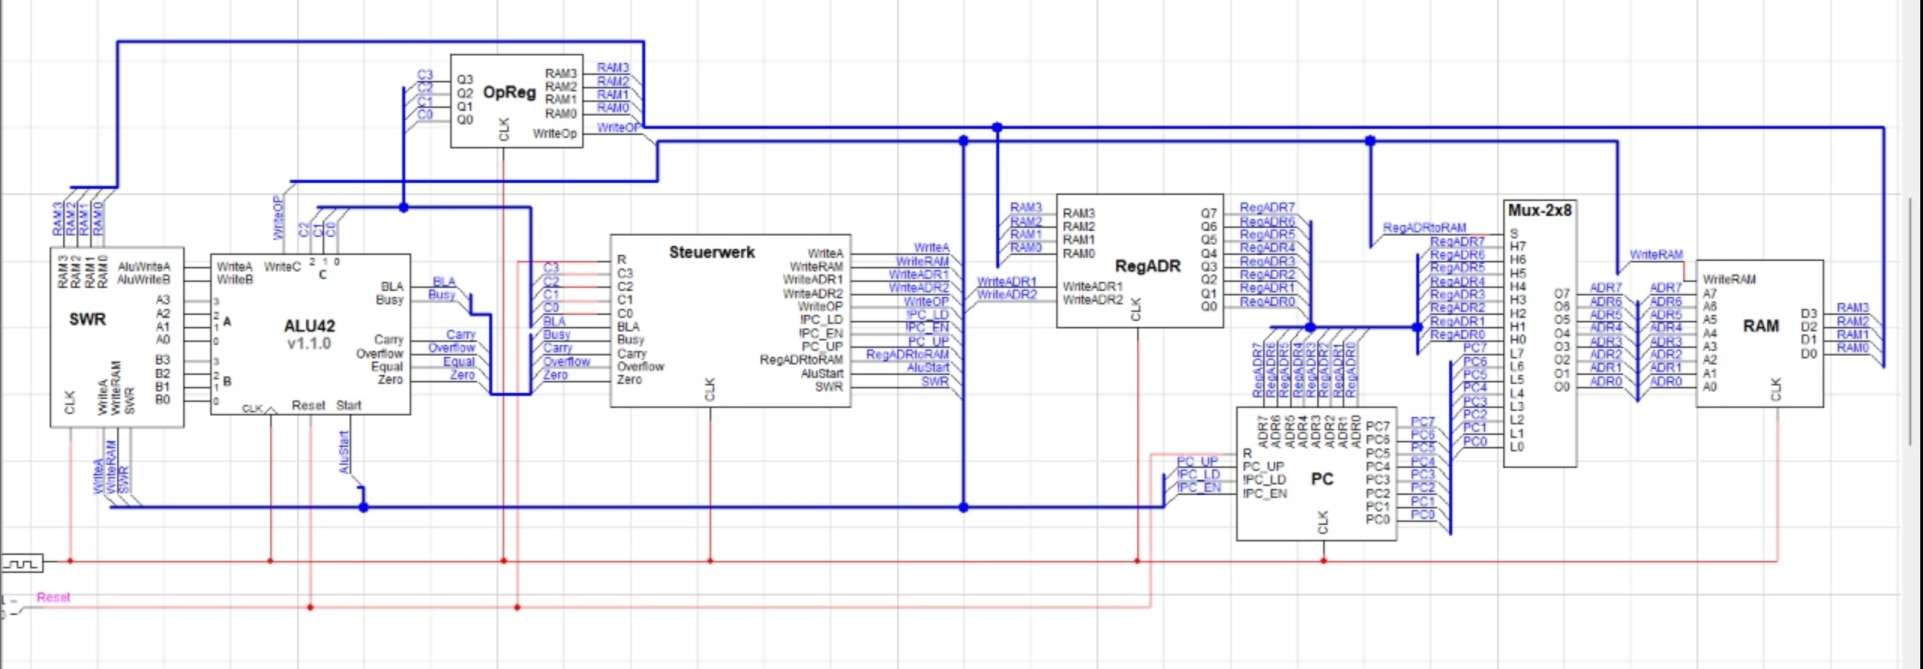
\includegraphics[scale=0.2]
    {content/figures/blockschaltbild-steuerwerk.jpg}
    \caption{LogicWorks Blockschaltbild Steuerwerk}
    \label{fig:lw-bsb-steuerwerk}
\end{figure}


\begin{figure}[ht]
    \centering
    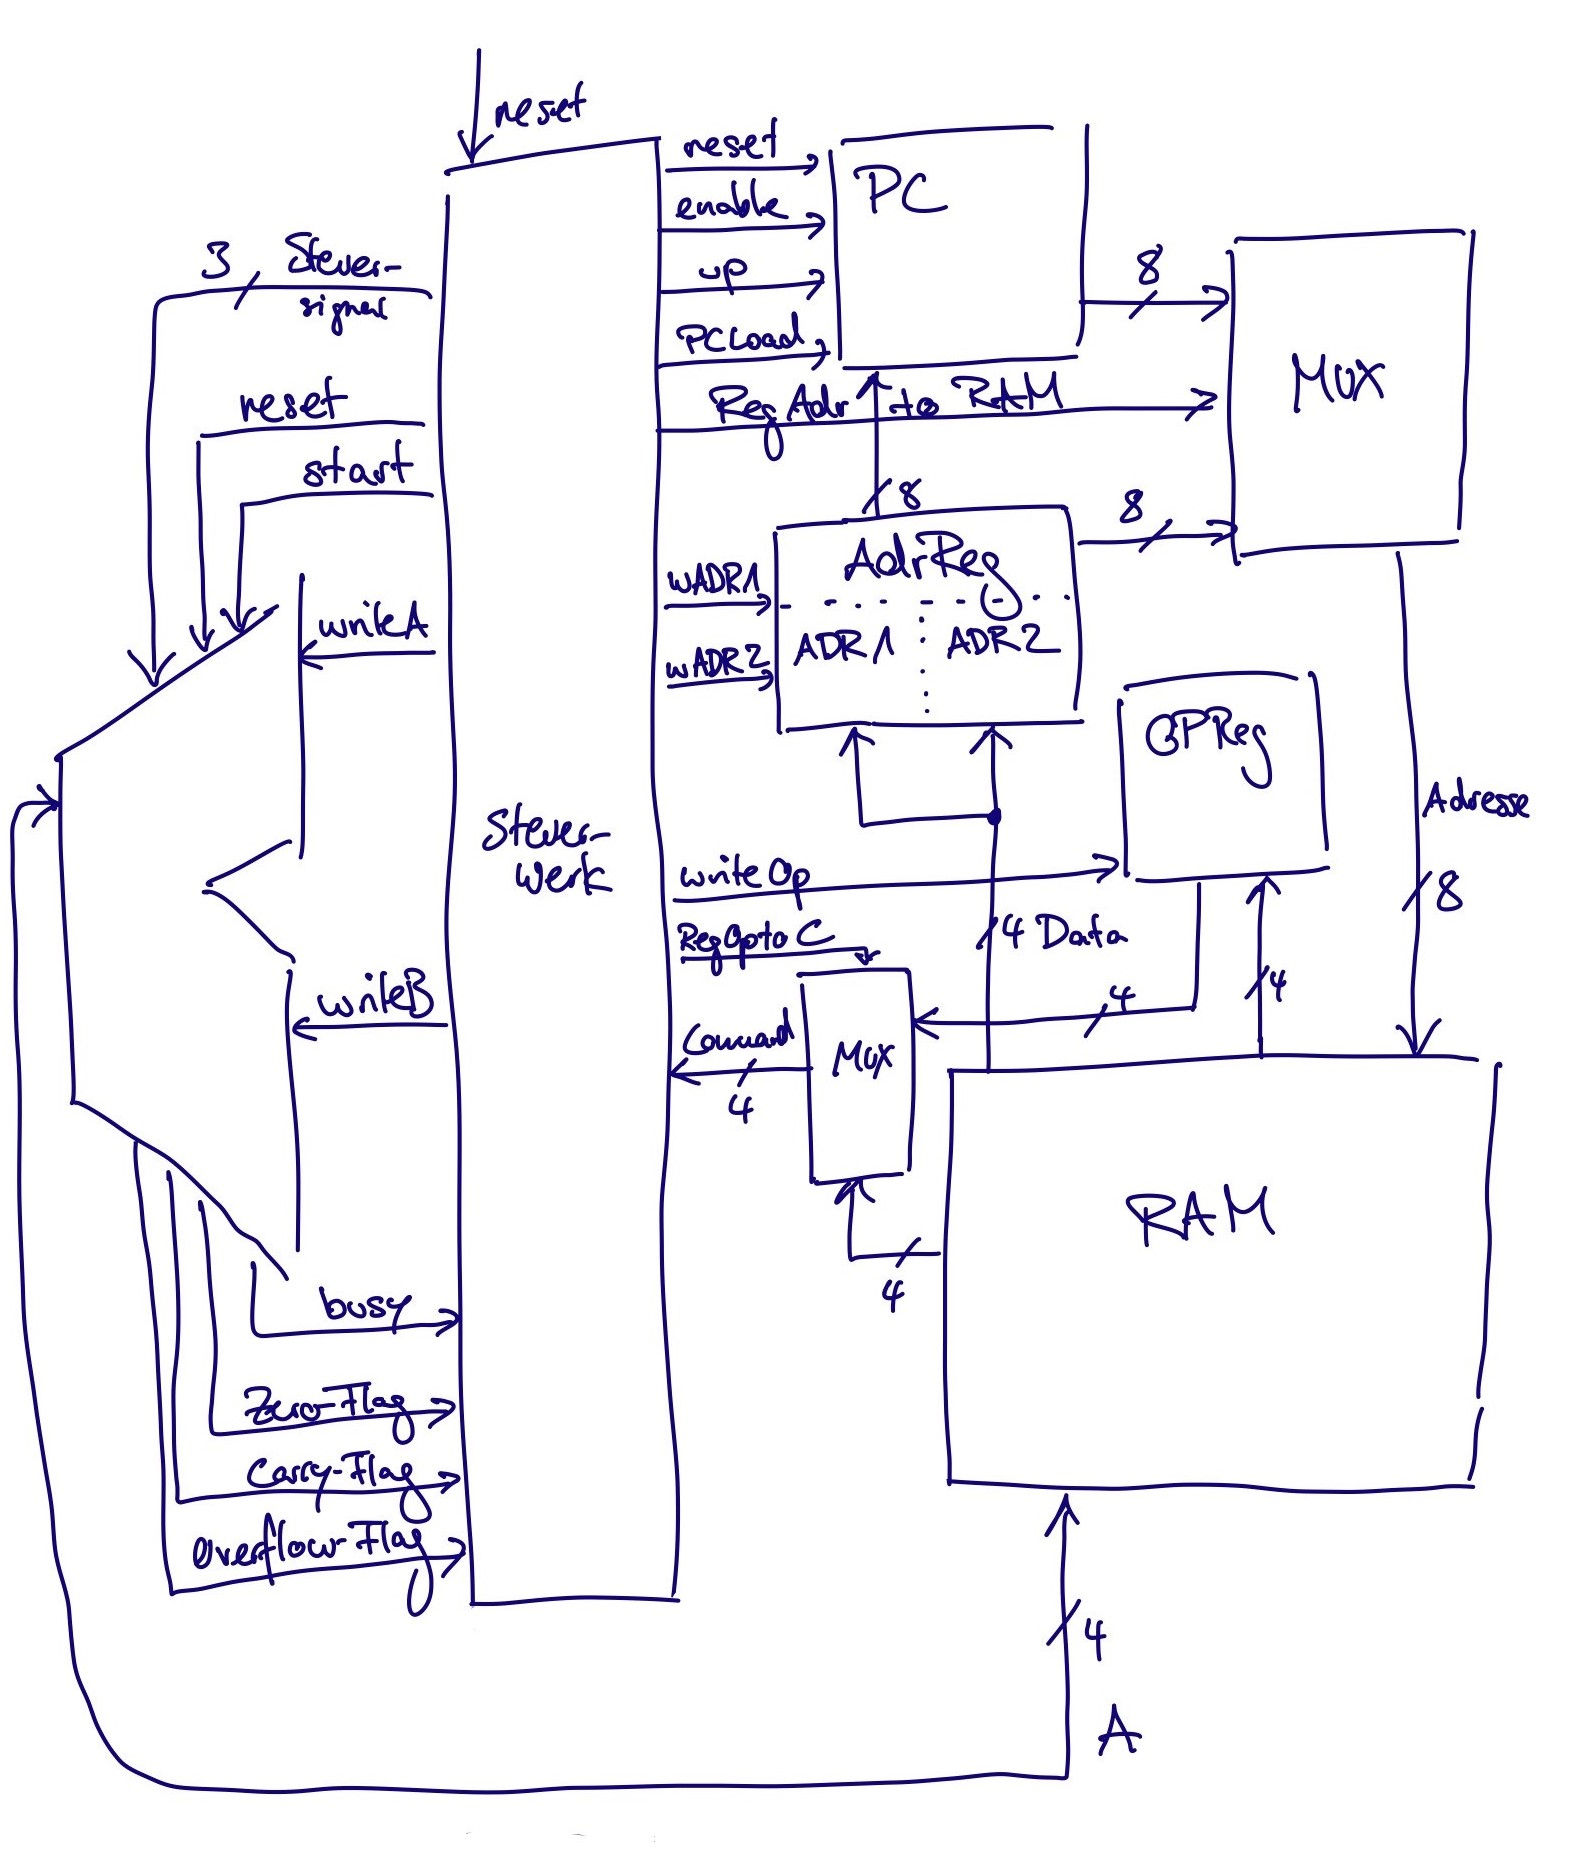
\includegraphics[scale=0.3]
    {content/figures/BSB_SW.jpg}
    \caption{First Level Blockschaltbild}
    \label{fig:blockschaltbild-first-level}
\end{figure}

\subsection{Transitionsfunktion Überführungsfunktion}
\label{sec:transitionsfunktion}

\begin{figure}[ht]
    \centering
    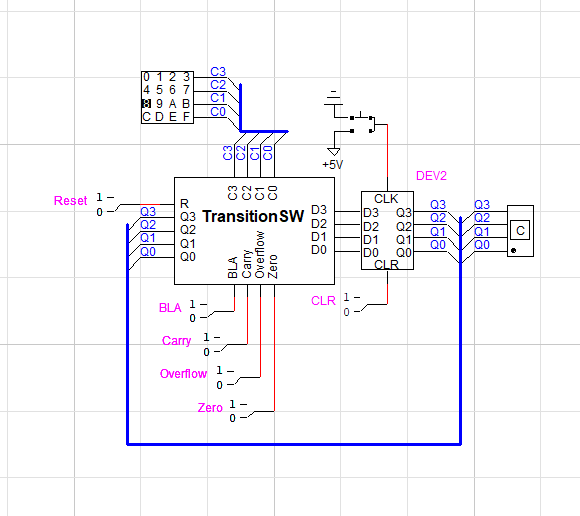
\includegraphics[scale=0.6]
    {content/figures/Transitionsfunktion.png}
    \caption{Blockschaltbild der Transitionsfunktion}
    \label{fig:blockschaltbild-transitionsfunktion}
\end{figure}

\begin{figure}[ht]
    \centering
    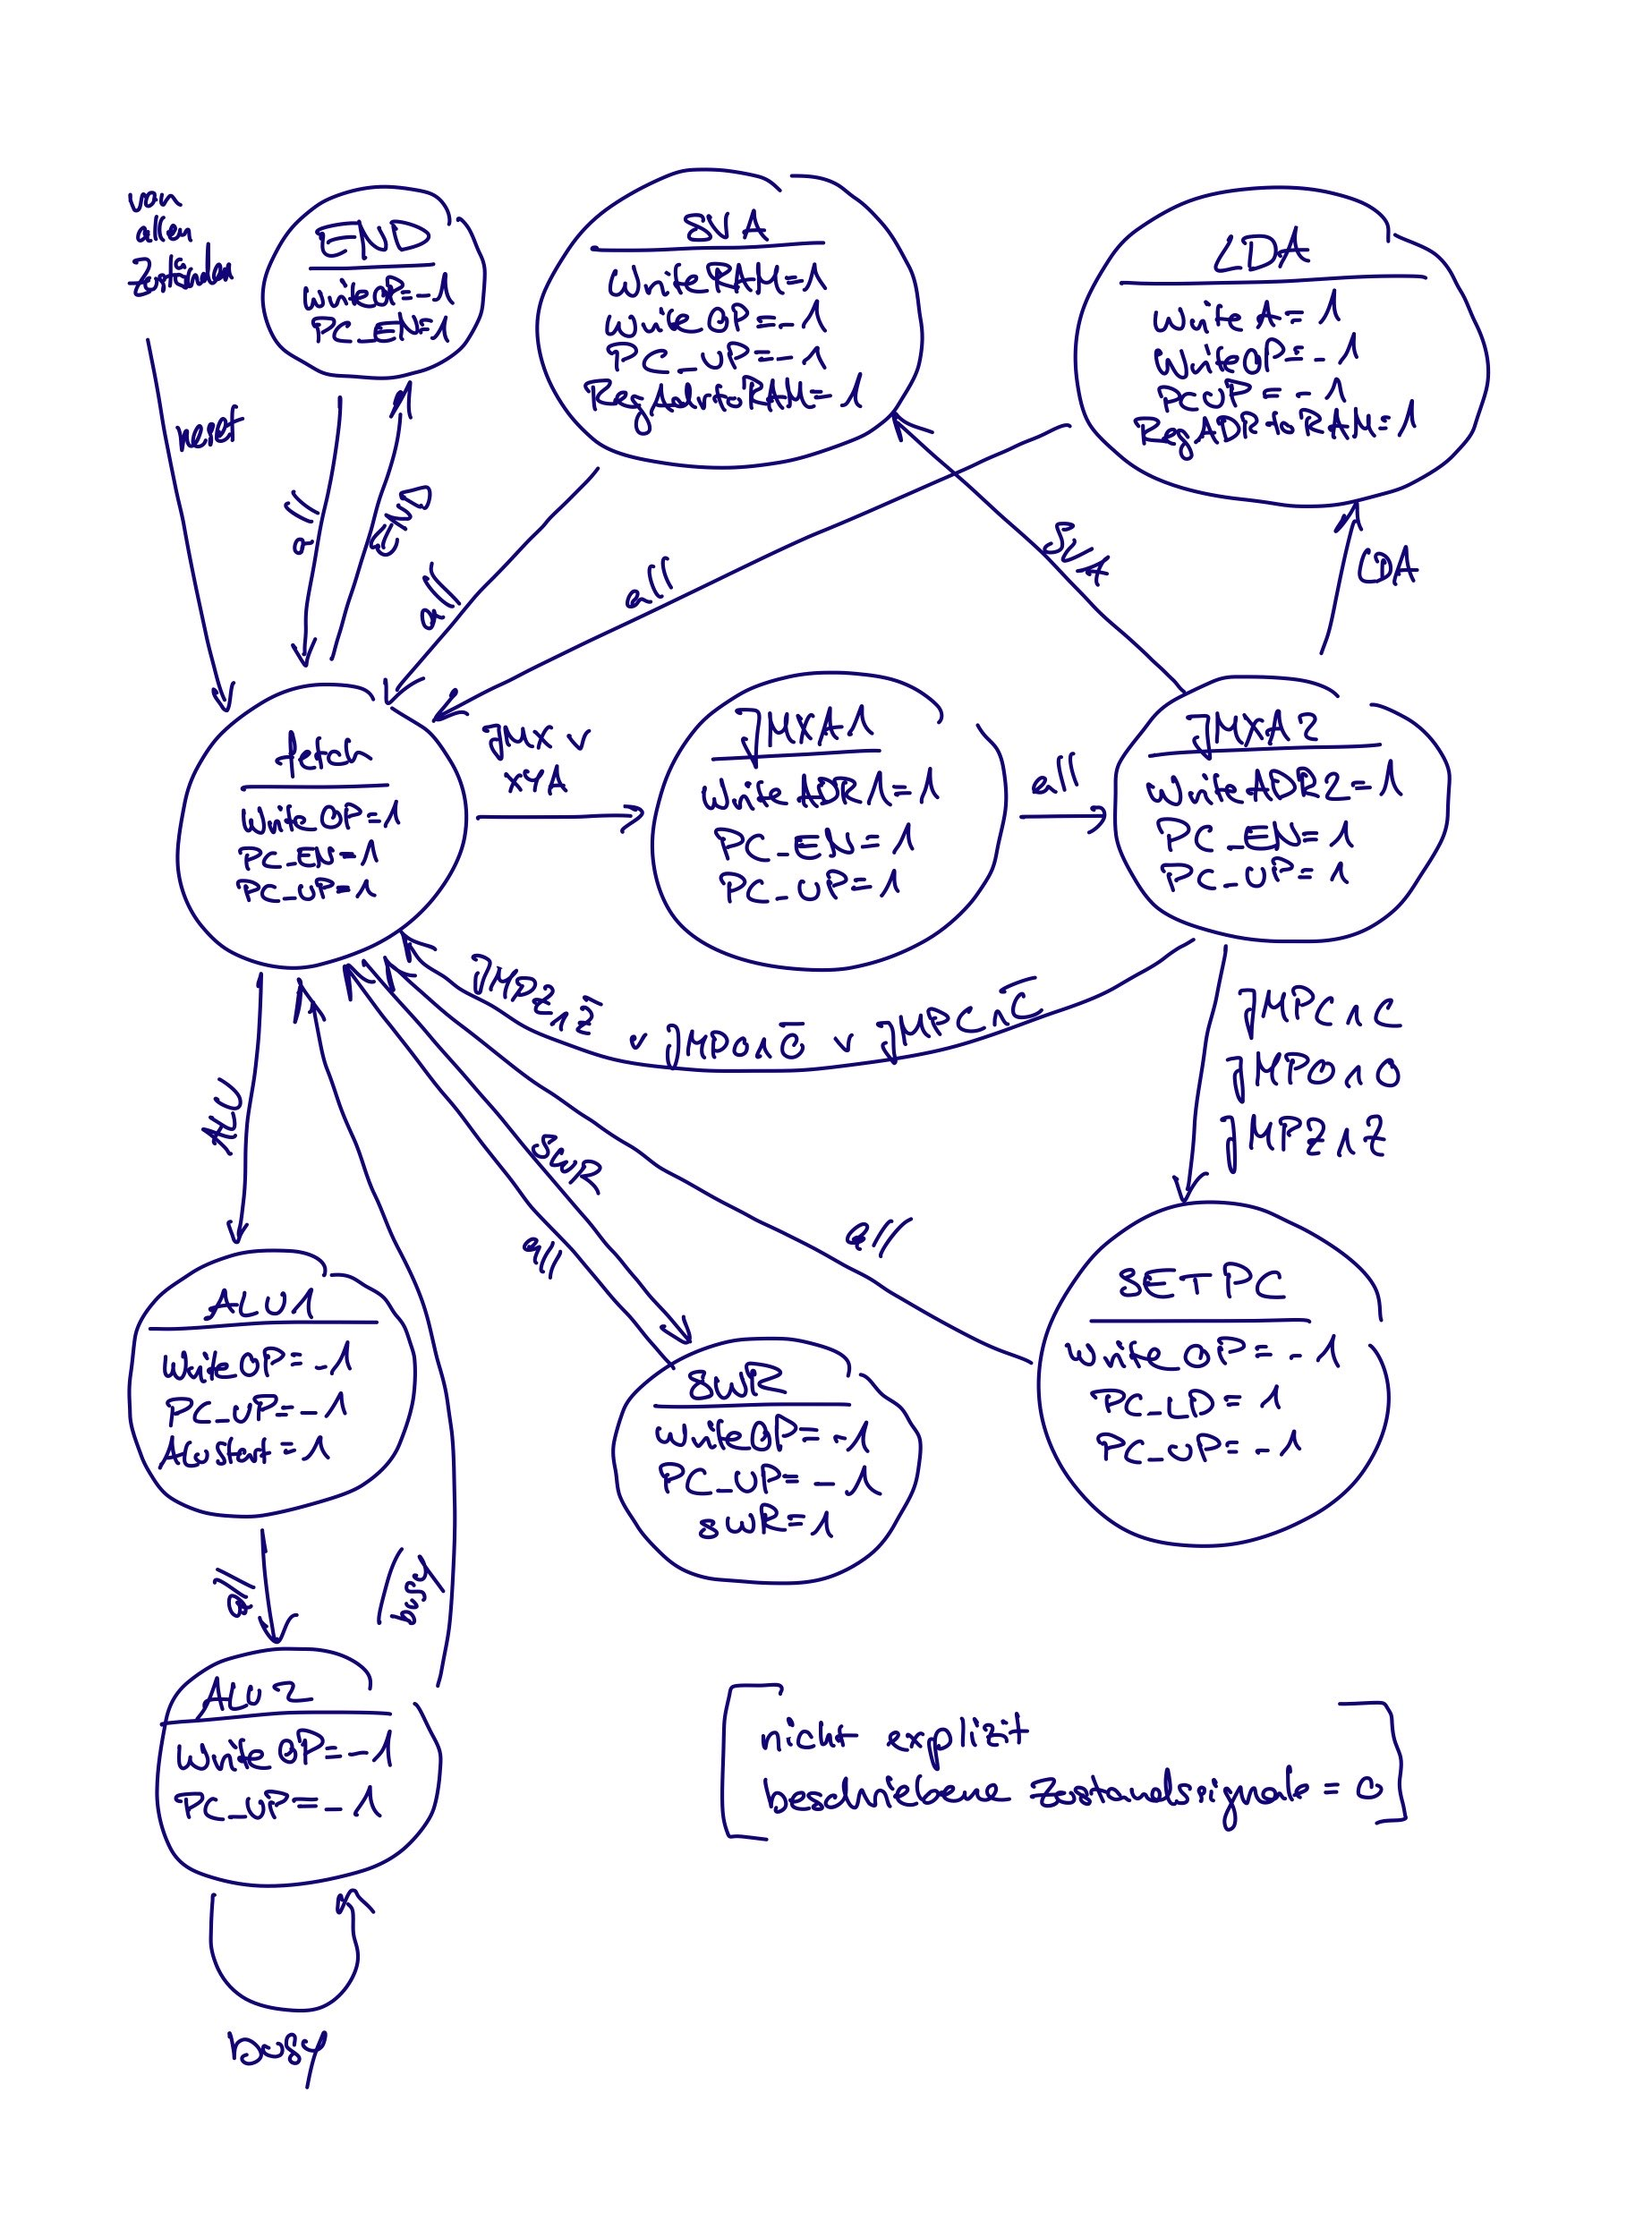
\includegraphics[scale=0.2]
    {content/figures/SW_Zustaende.jpg}
    \caption{Zustandsautomat Steuerwerk}
    \label{fig:SW_Zustaende}
\end{figure}

\subsection{Steuerwerk Ein und Ausgänge}
\label{sec:steuerwerk-ein-und-ausgänge}

\textbf{Eingänge}
\begin{itemize}
    \item Reset
    \item Q3..0
    \item BLA (Busy Look Ahead) und Busy
    \item Carry
    \item Overflow
    \item Zero
    \item Command
    \item C3..0
\end{itemize}


\textbf{Ausgänge}
\begin{itemize}
    \item WriteA: aus dem RAM in Register A der ALu schreiben
    \item WriteRAM: aus Register A in den RAM schreiben
    \item WriteADR1: in RegADR werden hiermit die MSBs geschrieben
    \item WriteADR2: in RegAdr werden hiermit die LSBs geschrieben
    \item WriteOP: die Operationen werden zwischengespeichert ins Operationsregister in der Fetchphase
    \item !PC-LD: die Programmcounter wird geladen
    \item !PC-EN: die Programmcounter zählt runter
    \item PC-UP: die Programmcounter wird hochgezählt
    \item RegADRtoRAM: im RAM wird die Adresse des RegAdr verwendet, anstatt die des Programm Counters
    \item ALUStart: die Funktionen der ALU werden durch diesen Befehl ausgeführt
    \item SWR: die Inhalte beider Adressen werden vertauscht
\end{itemize}

\subsection{RAM}
\label{sec:ram}



\subsection{Programm Counter}
\label{sec:programm-counter}

zählt die Operationen hoch, die ausgeführt wurden

\subsection{Adress Register}
\label{sec: adress-register}

Besteht aus zwei 2x4 Multiplexern, besteht aus zwei 2x4 Adressbits, werden für den RAM verwendet

\subsection{Operations Register}
\label{sec: operations-register}

\subsection{Steuerwerk}
\label{sec:steuerwerk}